%!TEX root=../oi-magistr-si.tex
\section[AOS - Kvalita, bezpečnost]{Architektura zaměřená na služby (SOA). Kvalita, výkonnost a škálování služeb. Zabezpečení, integrita, bezpečnost, a autentifikace služeb. Point-to-point a end-to-end šifrování.}

\url{http://www.w3c.or.kr/kr-office/TR/2003/ws-qos/}

\paragraph{Výkonnost}
Výkonnost reprezentuje jak rychle služba zpracuje dotaz. To může být měřeno dobou odezvy, dobou spouštění, nebo doby jednotlivých transakcí.

\paragraph{Spolehlivost}
Schopnost poskytnout službu na požádání uživatelem a poskytovat ji po požadovanou dobu v rámci specifikovaných tolerancí a dalších daných podmínek.

\paragraph{Škálovatelnost}
Schopnost zvyšování výpočetní kapacity za účelem zvýšení výkonnosti a kapacity. Služba by měla být škálovatelná ve smyslu navýšení počtu operací a transakcí.

\paragraph{Kapacita}
Služba by měla být poskytována s požadovanou kapacitou, tzn. garantovaným výkonem při zadaném počtu (kapacitě) paralelních requestů.

\paragraph{Robustnost}
Robustnost značí schopnost správného fungovaní služby i při nevalidních (nekompetních, konfliktních) vstupech.

\paragraph{Zpracování výjimek}
Služby by měli být poskytovány s funkcionalitou zpracování chyb a výjimek.

\paragraph{Integrita}
Služba umí předcházet/bránit neopravněnému přistupu nebo modifikaci k datům. Jsou dva typy integrity: datová a transakční.

\paragraph{Přístupnost}
Přistupnost je schopnost obsluhovat klientské požadavky (requesty). Dostupnost se dá navýšit vytvářením škálovatelných služeb.

\paragraph{Dostupnost}
Chceme co nejvyšší dostupnost služby, jako parametr se udává Time-to-Repair (TTR).

\paragraph{Bezpečnost}
Service Security Performance - Odolnost proti neoprávněnému odposlechu, neoprávněnému použití, zlovolnému poškození, nesprávnému použití, lidským chybám a přírodním katastrofám.

\subsection{Bezpečnost}
Poskytuje se bezpečnost klienta, serveru a zpráv. Bezpečnost zpráv je pokryta kryptografií (symetrické/asymetrické šifrování, digitální podpisy a certifikáty). U bezpečnosti klienta je řešeno: service discovery risk, phishing risk, autenticita a korektnost přijatých zpráv, autentikace poskytovatelů služeb. A zabezpečení serveru je řešení pomocí zabezpečení přenosového kanálu (HTTPS,SSL,SSH).


\paragraph{Point-to-point}
\hl{Communication channel level zabezpečení}. Guarantied on the server basis
\begin{figure}[h!]
\centering
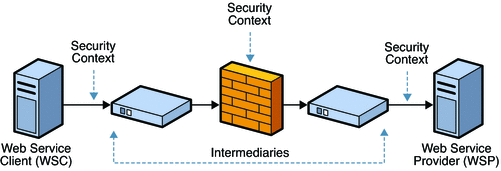
\includegraphics[width=80mm]{12/images/security-p2p}
\end{figure}

\paragraph{End-to-end}
\hl{Message level zabezpečení}. Application oriented security

\begin{figure}[h!]
\centering
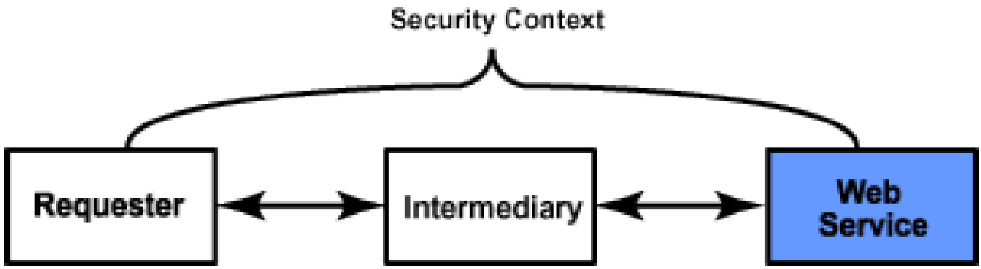
\includegraphics[width=80mm]{12/images/security-e2e}
\end{figure}

\begin{itemize}[itemsep=0px]
\item \textbf{XML signatura} - Podepisuje se buď celý dokument, nebo jen část
\item \textbf{XML šifrování} - end-to-end, v soap obálce je oddíl se security tokenem a signaturou.
\end{itemize}
